\documentclass[11pt,preprint, authoryear]{elsarticle}

\usepackage{lmodern}
%%%% My spacing
\usepackage{setspace}
\setstretch{1.2}
\DeclareMathSizes{12}{14}{10}{10}

% Wrap around which gives all figures included the [H] command, or places it "here". This can be tedious to code in Rmarkdown.
\usepackage{float}
\let\origfigure\figure
\let\endorigfigure\endfigure
\renewenvironment{figure}[1][2] {
    \expandafter\origfigure\expandafter[H]
} {
    \endorigfigure
}

\let\origtable\table
\let\endorigtable\endtable
\renewenvironment{table}[1][2] {
    \expandafter\origtable\expandafter[H]
} {
    \endorigtable
}


\usepackage{ifxetex,ifluatex}
\usepackage{fixltx2e} % provides \textsubscript
\ifnum 0\ifxetex 1\fi\ifluatex 1\fi=0 % if pdftex
  \usepackage[T1]{fontenc}
  \usepackage[utf8]{inputenc}
\else % if luatex or xelatex
  \ifxetex
    \usepackage{mathspec}
    \usepackage{xltxtra,xunicode}
  \else
    \usepackage{fontspec}
  \fi
  \defaultfontfeatures{Mapping=tex-text,Scale=MatchLowercase}
  \newcommand{\euro}{€}
\fi

\usepackage{amssymb, amsmath, amsthm, amsfonts}

\def\bibsection{\section*{References}} %%% Make "References" appear before bibliography


\usepackage[round]{natbib}

\usepackage{longtable}
\usepackage[margin=2.3cm,bottom=2cm,top=2.5cm, includefoot]{geometry}
\usepackage{fancyhdr}
\usepackage[bottom, hang, flushmargin]{footmisc}
\usepackage{graphicx}
\numberwithin{equation}{section}
\numberwithin{figure}{section}
\numberwithin{table}{section}
\setlength{\parindent}{0cm}
\setlength{\parskip}{1.3ex plus 0.5ex minus 0.3ex}
\usepackage{textcomp}
\renewcommand{\headrulewidth}{0.2pt}
\renewcommand{\footrulewidth}{0.3pt}

\usepackage{array}
\newcolumntype{x}[1]{>{\centering\arraybackslash\hspace{0pt}}p{#1}}

%%%%  Remove the "preprint submitted to" part. Don't worry about this either, it just looks better without it:
\makeatletter
\def\ps@pprintTitle{%
  \let\@oddhead\@empty
  \let\@evenhead\@empty
  \let\@oddfoot\@empty
  \let\@evenfoot\@oddfoot
}
\makeatother

 \def\tightlist{} % This allows for subbullets!

\usepackage{hyperref}
\hypersetup{breaklinks=true,
            bookmarks=true,
            colorlinks=true,
            citecolor=blue,
            urlcolor=blue,
            linkcolor=blue,
            pdfborder={0 0 0}}


% The following packages allow huxtable to work:
\usepackage{siunitx}
\usepackage{multirow}
\usepackage{hhline}
\usepackage{calc}
\usepackage{tabularx}
\usepackage{booktabs}
\usepackage{caption}


\newenvironment{columns}[1][]{}{}

\newenvironment{column}[1]{\begin{minipage}{#1}\ignorespaces}{%
\end{minipage}
\ifhmode\unskip\fi
\aftergroup\useignorespacesandallpars}

\def\useignorespacesandallpars#1\ignorespaces\fi{%
#1\fi\ignorespacesandallpars}

\makeatletter
\def\ignorespacesandallpars{%
  \@ifnextchar\par
    {\expandafter\ignorespacesandallpars\@gobble}%
    {}%
}
\makeatother

\newlength{\cslhangindent}
\setlength{\cslhangindent}{1.5em}
\newenvironment{CSLReferences}%
  {\setlength{\parindent}{0pt}%
  \everypar{\setlength{\hangindent}{\cslhangindent}}\ignorespaces}%
  {\par}


\urlstyle{same}  % don't use monospace font for urls
\setlength{\parindent}{0pt}
\setlength{\parskip}{6pt plus 2pt minus 1pt}
\setlength{\emergencystretch}{3em}  % prevent overfull lines
\setcounter{secnumdepth}{5}

%%% Use protect on footnotes to avoid problems with footnotes in titles
\let\rmarkdownfootnote\footnote%
\def\footnote{\protect\rmarkdownfootnote}
\IfFileExists{upquote.sty}{\usepackage{upquote}}{}

%%% Include extra packages specified by user

%%% Hard setting column skips for reports - this ensures greater consistency and control over the length settings in the document.
%% page layout
%% paragraphs
\setlength{\baselineskip}{12pt plus 0pt minus 0pt}
\setlength{\parskip}{12pt plus 0pt minus 0pt}
\setlength{\parindent}{0pt plus 0pt minus 0pt}
%% floats
\setlength{\floatsep}{12pt plus 0 pt minus 0pt}
\setlength{\textfloatsep}{20pt plus 0pt minus 0pt}
\setlength{\intextsep}{14pt plus 0pt minus 0pt}
\setlength{\dbltextfloatsep}{20pt plus 0pt minus 0pt}
\setlength{\dblfloatsep}{14pt plus 0pt minus 0pt}
%% maths
\setlength{\abovedisplayskip}{12pt plus 0pt minus 0pt}
\setlength{\belowdisplayskip}{12pt plus 0pt minus 0pt}
%% lists
\setlength{\topsep}{10pt plus 0pt minus 0pt}
\setlength{\partopsep}{3pt plus 0pt minus 0pt}
\setlength{\itemsep}{5pt plus 0pt minus 0pt}
\setlength{\labelsep}{8mm plus 0mm minus 0mm}
\setlength{\parsep}{\the\parskip}
\setlength{\listparindent}{\the\parindent}
%% verbatim
\setlength{\fboxsep}{5pt plus 0pt minus 0pt}



\begin{document}



\begin{frontmatter}  %

\title{Question 5}

% Set to FALSE if wanting to remove title (for submission)




\author[Add1]{Joshua Strydom\footnote{\textbf{Contributions:}
  \newline \emph{The authors would like to thank no institution for
  money donated to this project. Thank you sincerely.}}}
\ead{20718284@sun.ac.za}





\address[Add1]{Stellenbosch University, Stellenbosch, South Africa}



\vspace{1cm}





\vspace{0.5cm}

\end{frontmatter}



%________________________
% Header and Footers
%%%%%%%%%%%%%%%%%%%%%%%%%%%%%%%%%
\pagestyle{fancy}
\chead{}
\rhead{}
\lfoot{}
\rfoot{\footnotesize Page \thepage}
\lhead{}
%\rfoot{\footnotesize Page \thepage } % "e.g. Page 2"
\cfoot{}

%\setlength\headheight{30pt}
%%%%%%%%%%%%%%%%%%%%%%%%%%%%%%%%%
%________________________

\headsep 35pt % So that header does not go over title




\hypertarget{introduction}{%
\section{\texorpdfstring{Introduction
\label{Introduction}}{Introduction }}\label{introduction}}

\begin{figure}[H]

{\centering \includegraphics{Question5_files/figure-latex/Figure1-1} 

}

\caption{Caption Here \label{Figure1}}\label{fig:Figure1}
\end{figure}

Figure \ref{Figure1} displays the price changes for the various
currencies. South Africa, although not the most volatile, is relatively
volatile to many currencies.

\begin{figure}[H]

{\centering \includegraphics{Question5_files/figure-latex/Figure2-1} 

}

\caption{Caption Here \label{Figure2}}\label{fig:Figure2}
\end{figure}

Figure \ref{Figure2} plots the standard deviation of simple returns and
clearly shows that South Africa is not the most volatile currency in the
BRICS.

\begin{figure}[H]

{\centering \includegraphics{Question5_files/figure-latex/Figure3-1} 

}

\caption{Caption Here \label{Figure3}}\label{fig:Figure3}
\end{figure}

Figure \ref{Figure3}, however, shows South Africa to be the more
volatile currency when compared to G10 member countries in the sample.

\hypertarget{simple-rolling-standard-deviation-calculation-for-south-africas-currency-volatility}{%
\section{Simple rolling standard deviation calculation for South
Africa's currency
volatility}\label{simple-rolling-standard-deviation-calculation-for-south-africas-currency-volatility}}

\begin{figure}[H]

{\centering \includegraphics{Question5_files/figure-latex/Figure4-1} 

}

\caption{Caption Here \label{Figure4}}\label{fig:Figure4}
\end{figure}

\hypertarget{currency-carry-trades}{%
\section{\texorpdfstring{Currency carry trades
\label{carry}}{Currency carry trades }}\label{currency-carry-trades}}

\begin{figure}[H]

{\centering \includegraphics{Question5_files/figure-latex/Figure5-1} 

}

\caption{Caption Here \label{Figure5}}\label{fig:Figure5}
\end{figure}

Figure \ref{Figure5} shows the simple return of both the South African
currency and the carry currency. It can be noted that the Rand follows
the currency carry and has performed well during periods where G10
currency carry trades have been favourable. Globally, it has been one of
the currencies that most benefit during periods where the Dollar is
comparatively strong.

\hypertarget{implied-volatility}{%
\section{\texorpdfstring{Implied volatility
\label{IV}}{Implied volatility }}\label{implied-volatility}}

\begin{figure}[H]

{\centering \includegraphics{Question5_files/figure-latex/Figure6-1} 

}

\caption{Caption Here \label{Figure6}}\label{fig:Figure6}
\end{figure}

Figure \ref{Figure6} shows the log returns of implied volatility. The
most volatile of the group are that of Brazil, China, India and South
Africa.

\begin{figure}[H]

{\centering 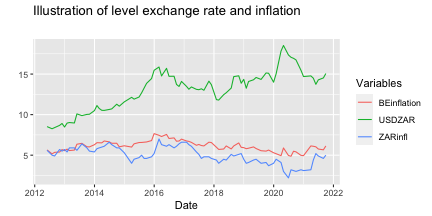
\includegraphics{Question5_files/figure-latex/Figure7-1} 

}

\caption{Caption Here \label{Figure7}}\label{fig:Figure7}
\end{figure}

Figure \ref{Figure7} again shows South Africa to have a high relative
implied volatility.

\begin{figure}[H]

{\centering \includegraphics{Question5_files/figure-latex/Figure8-1} 

}

\caption{Caption Here \label{Figure8}}\label{fig:Figure8}
\end{figure}

Figure \ref{Figure8} shows South Africa to have the highest implied
volatility relative to the G10 member states in the data provided.

\hypertarget{conclusion}{%
\section{\texorpdfstring{Conclusion
\label{Concl}}{Conclusion }}\label{conclusion}}

The South African rand (ZAR) has over the past few years been one of the
most volatile currencies.

\bibliography{Tex/ref}





\end{document}
